\documentclass[english,12pt]{aghthesis}

\usepackage[T1]{fontenc}
\usepackage[utf8]{inputenc}
\usepackage{upgreek}
\usepackage{polski}
\usepackage{url}
\usepackage{tikz}
\usepackage{graphicx}
\usepackage{float}
\usepackage{hyperref}

\author{Antoni Mleczko \\ Maciej Mionskowski}

\titlePL{Interaktywna wizualizacja instrukcji składania Origami z elementami symulacji fizyki papieru}
\titleEN{Interactive visualisation of Origami folding with elements of paper physics simulation}

\fieldofstudy{Informatyka}

\supervisor{dr inż. Witold Alda}

\date{\the\year}

\begin{document}
\setlength{\parskip}{0pt} % 1ex plus 0.5ex minus 0.2ex}
\setlength{\parindent}{0pt}

\maketitle

\section{\SectionTitleProjectVision}
\label{sec:cel-wizja}

\subsection{Problem characteristics}
Origami has been around for a long time. It originated in China and Japan, roughly at the same time, from where it 
spread all around the world\cite{wiki:history-of-origami}. 
Origami is recognized as the art of paper folding.
Although known for centuries, it exhibits properties that are applicable 
in many different contemporary contexts, e.g.
space exploration\cite{origami-in-orbit}, or deploying solar arrays\cite{solar-panel-origami}.
It has recently started to attract attention among scientists and engineers.
Researchers are now recognizing material folding as a distinct
branch of computer science, known as \hyperref[dictionary:computational-origami]{\textit{computational origami}}.
The field has seen tremendous development in the past couple of decades.
Being such a broad topic, it is not surprising that there are numerous open problems\cite{mit-open-problems} and on-going research.

\medskip

While beginners fold origami following step-by-step instructions,
more advanced origamists would use \hyperref[dictionary:crease-pattern]{\textit{crease patterns}}
to form the \hyperref[dictionary:folded-state]{\textit{folded state}}.
The process of origami creation consists of two stages: \textit{design} and \textit{folding}.
The former is a reference to the \textit{crease pattern} creation, and the latter is the process of the actual folding.

\begin{figure}[H]
\caption{A crease pattern for a popular origami model, a crane.\label{fig:creasepattern}}
  \centering
    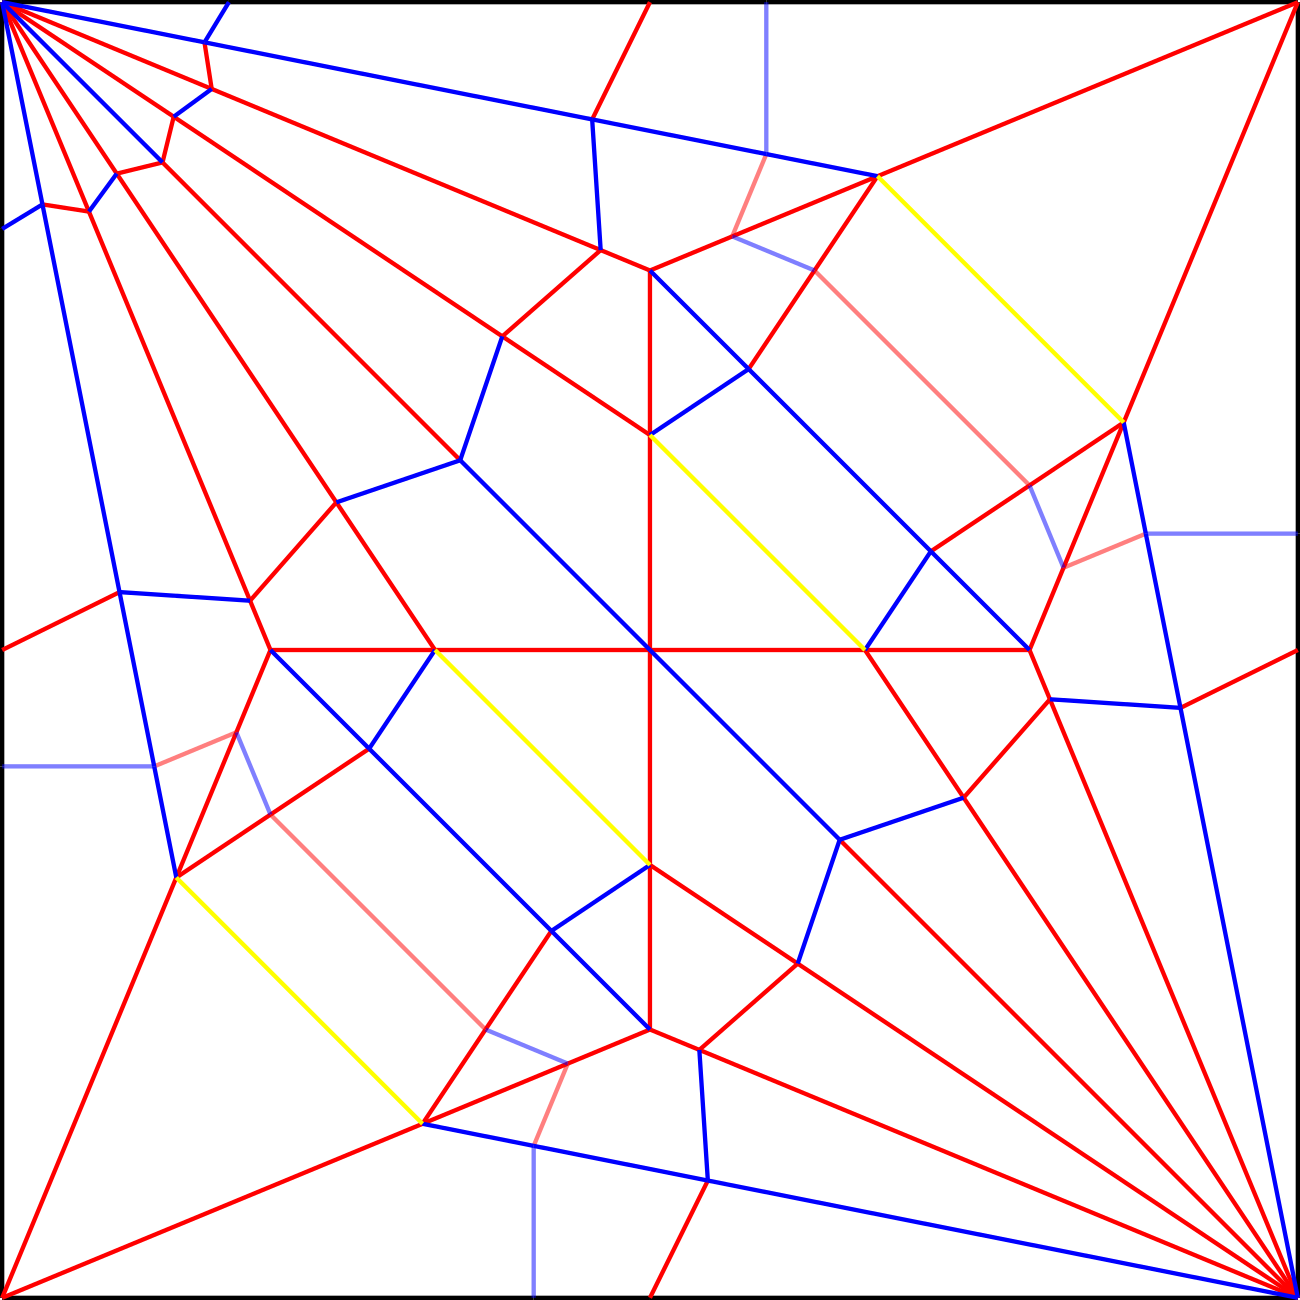
\includegraphics[width=0.8\textwidth]{assets/crane-crease-pattern.png}
\end{figure}

\subsection{Motivation}

Even though origami might seem to be a child's play, at times
people would get discouraged whilst following the origami instructions due to
the lack of details they expose.

We would like to provide a way, for beginners and advanced origamists alike,
to visualize the folding process step by step.
While there exist some programs aiding the process of design\cite{app:treemaker}\cite{app:omto}\cite{app:origami-draw}, there is no satisfactory solution 
that would present the process of folding the way it would be carried out manually.

We have evaluated existing products, and the one that resembles 
what we would like to achieve the most\cite{origami-simulator} provides a way to load a crease pattern
and view the folding process. 
However, it goes immediately from a flat sheet of paper to the folded figure, skipping all the steps
that would be required while folding the figure by hand.
It also bypasses some physical properties that we would like to achieve, such as the fact that the
paper should not interpenetrate itself.


\begin{figure}[H]
\caption{Origami simulator by Amanda Ghassaei}
  \centering
    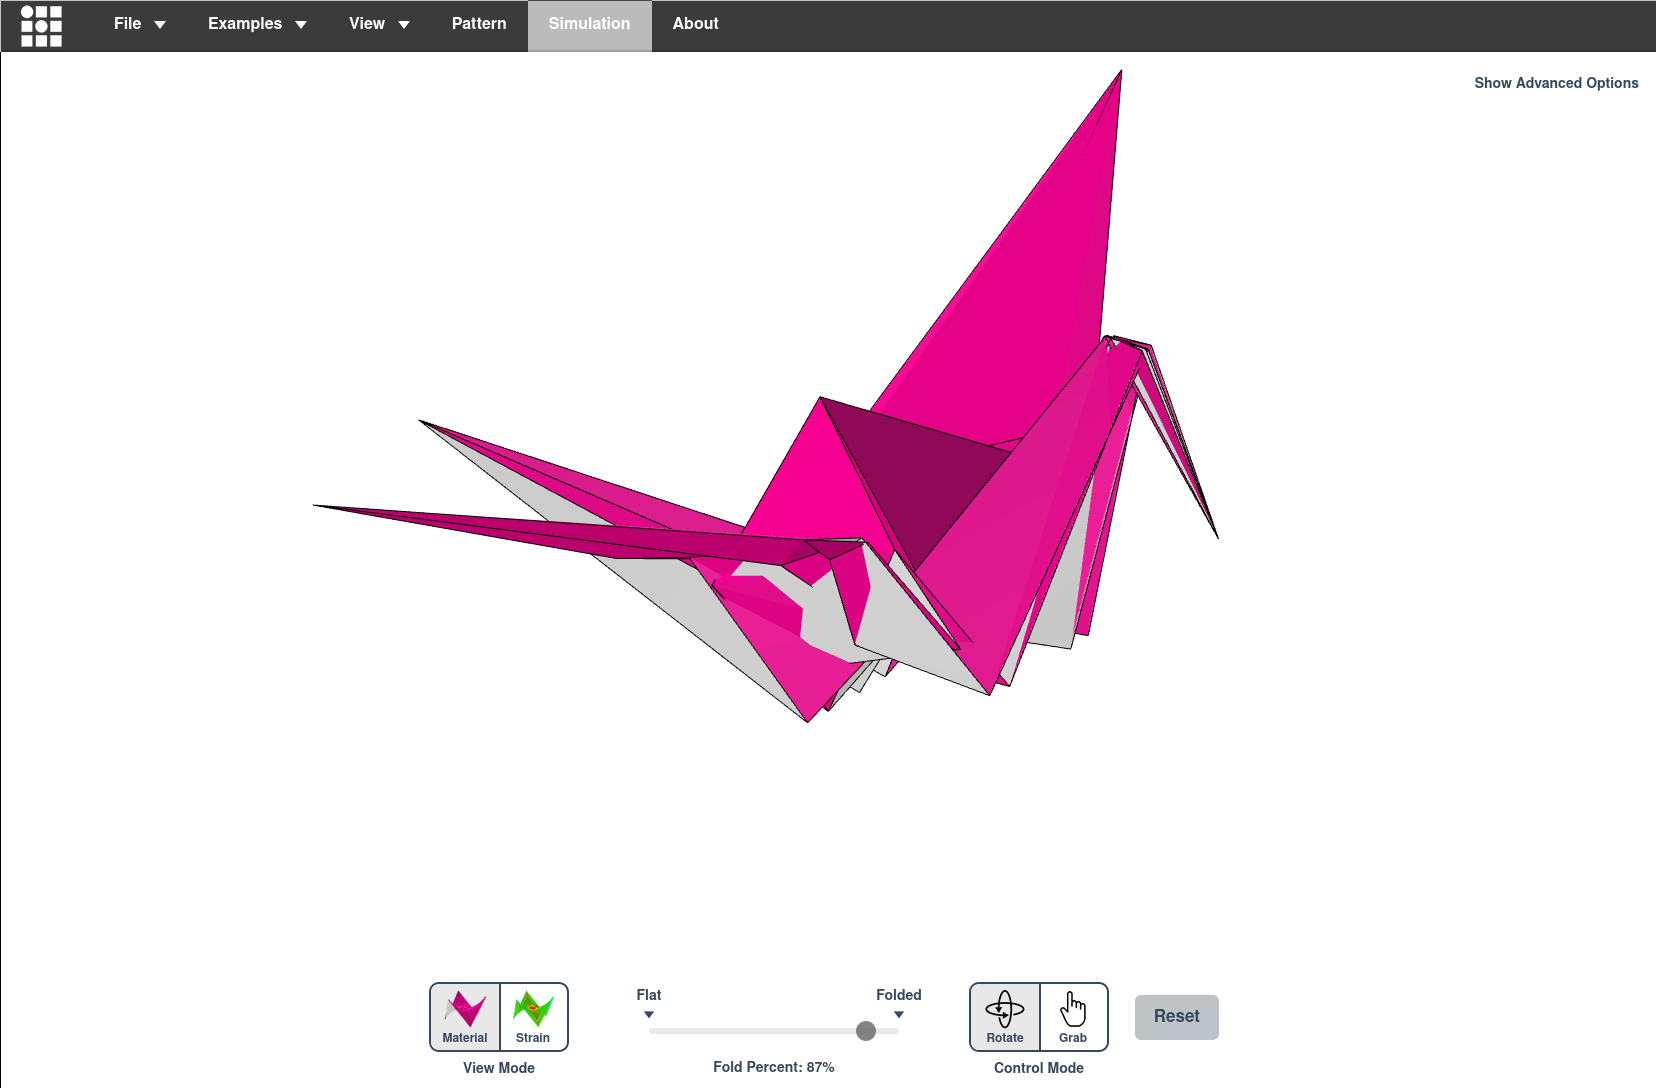
\includegraphics[width=\textwidth]{assets/origami-simulator.png}
\end{figure}

\clearpage 

\subsection{Product Vision}

\subsubsection{Functionality}

Our main goal is to create a platform that would allow visualisation of the origami folding process in a 3D space.
It would be possible to see how the figure folds at each step by playing an animation of the transition.

The inseparable component of the system would be a file format describing the folding sequence necessary to complete the origami figure.\\

The users in our system would at least be able to:
\begin{itemize}
	\item load a folding instruction,
	\item choose a step they want visualized,
	\item rotate the scene,
    \item zoom in and out,
	\item move around the scene,
	\item pause the animation at any time, and move back and forth.
\end{itemize}

\subsubsection{Technology}

Our application will consist of two layers -- backend and frontend.

The backend part will be responsible for storing user files and turning Instructions into animated Guides.
The frontend part will handle user interactions and 3D visualisations.

We have decided to use well-known and widely spread technologies.
For the backend part we will take advantage of \tech{Python} language with \tech{Django} framework.
As a data storage, we are going to incorporate \tech{PostgreSQL}.

For the frontend, we will use \tech{JavaScript} with \tech{React} for building the user interface.
The 3D rendering will be performed using \tech{Three.js} library that is built on top of \tech{WebGL} renderer.

\begin{figure}[H]
	\caption{Technology stack}
	\centering
	\begin{tikzpicture}
	\node (backend) at (0,0) [draw,thick,minimum width=4cm,label=north west:Backend] {
		
\includegraphics[width=.15\textwidth]{assets/python.png}
		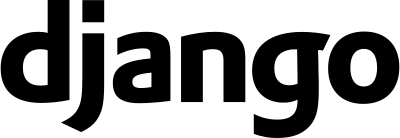
\includegraphics[width=.15\textwidth]{assets/django-logo.png}
	};
	\node[below = of backend] (frontend) [draw,thick,minimum width=4cm, label=north west:Frontend] {
		
\includegraphics[width=.12\textwidth]{assets/javascript-logo.png}
		
\includegraphics[width=.12\textwidth]{assets/react-logo.png}
		
\includegraphics[width=.23\textwidth]{assets/three-js-logo.png}
	};
	\draw[<->,thick] (backend.south) -- (frontend.north);
	\end{tikzpicture}
\end{figure}


\subsection{Feasibility Study}

Both \tech{Python} and \tech{JavaScript} are widely spread and actively maintained.
There is a strong community surrounding both of them.
\tech{Three.js} is the most popular library for 3D \tech{WebGL} rendering.

Therefore, we are not expecting problems connected with the tools we have selected.

Since the project will require a lot of knowledge from the \textit{computational origami}
field, we will have to research the existing materials on this topic.
The most promising resources seem to be the MIT course by
Eric Demaine\cite{mit-course} and a book co-authored by the same person -- \textit{Geometric Folding Algorithms: Linkages, Origami, Polyhedra}\cite{origami-book}.
Various available papers might come in handy as well, especially the ones regarding software implementations of origami folding algorithms.


\subsection{Threat Assessment}

Playing with the intersection between reality and computer science has always been a challenging task.
As the field of \textit{computational origami} is relatively young\cite{recent-results-in-computational-origami:paper}, there are still many obstacles to overcome.
As of now, the mathematical rules governing the origami folding are not fully developed.
On top of it, we are going to tackle a problem that has not been widely discussed.

Taking all of that into account, we foresee many challenges along the way, such as:

\begin{itemize}
	\item NP-hardness - some problems that we will face are proved to be NP-hard.
		Computing layer ordering based on a crease pattern is an example of such a problem.
		We will have to overcome them, either by using approximate methods or coming up with solutions that will avoid them.

	\item Physical properties of paper - should we support more complex physical properties,
		there are many features that would require a separate set of computations simulating paper physics, e.g.
		\begin{itemize}
			\item inflating,
			\item curving,
			\item cutting.
		\end{itemize}

	\item Performance -- web browsers are still not fully optimized to carry out 3D computations and render 3D graphics in real time.
		The system will have to be highly optimized in order to be usable.
		
	\item Mathematics -- we have little experience writing complex simulations utilizing complicated mathematical formulas.
		Even modelling a simple paper fold requires a lot of knowledge on different physical properties and frameworks that one could use.

	\item 3D graphics -- we have some experience working with 3D, however only from the user perspective.
		We have little experience in creating 3D graphical software.

\end{itemize}

Having said that, we believe we are capable of undertaking this problem and providing a solution to it.
Albeit challenging, it is rewarding especially in terms of projected business value and gained expertise.

\subsection{Dictionary}\label{dictionary}

\begin{description}
	\item[computational origami] \label{dictionary:computational-origami} -- a recent branch of computer science studying efficient algorithms for solving paper-folding problems.\cite{recent-results-in-computational-origami:paper}
	\item[crease] -- a line segment, along which a sheet of paper folds.
	\item[crease pattern] \label{dictionary:crease-pattern} -- a pattern of lines formed by creases that is created after unfolding the origami flat. For an example see figure \ref{fig:creasepattern}.
	\item[folded state] \label{dictionary:folded-state} -- An assembled origami model. Or alternatively, a sheet of paper folded along the crease pattern.
	\item[mountain] -- a fold of paper along the crease, such that the facets on the sides of the crease are facing downwards.
					\begin{figure}[H]
						\caption{Example of a mountain crease}
						\centering
						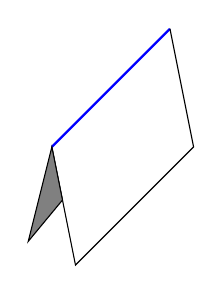
\begin{tikzpicture}[scale=1.5]
							\draw[blue, thick] (0,0) -- (1,1);
							\draw (1,1) -- (1.2, 0) --  (0.2, -1) -- (0,0);
							\filldraw[fill=gray] (0, 0) -- (-0.2, -0.8) -- (0.09, -0.45) -- cycle;
						\end{tikzpicture}
					\end{figure}
	\item[valley] -- A fold of paper along a crease, such that the facets on the sides of the crease are facing upwards.
					\begin{figure}[H]
						\caption{Example of a valley crease}
						\centering
						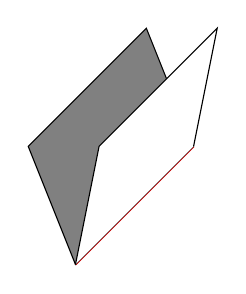
\begin{tikzpicture}[scale=1.5]
							\draw[red, thick] (0,0) -- (1,1);
							\filldraw[fill=gray] (0, 0) -- (-0.4, 1) -- (0.6, 2) -- (1, 1) -- cycle;
							\filldraw[fill=white] (1,1) -- (1.2, 2) --  (0.2, 1) -- (0,0);
						\end{tikzpicture}
					\end{figure}
	\item[mountain-valley assignment] -- an assignment of mountain or valley to the creases on the crease pattern.
	\item[.fold file] -- a file that conforms to the FOLD\cite{fold:paper} specification.
	\item[Instruction] -- a \textit{.fold} file created by a user, representing a sequence of steps required to
		fold a sheet of paper into a complete origami figure.
	\item[Transition] -- a folding animation played between two steps.
	\item[Guide] -- a set of all Transitions derived from an Instruction. Can be represented using a \textit{.fold} file.
	\item[Model] -- 3D representation of an origami figure. 
	\item[FPS] -- frames per second.
	\item[target angle] -- the supplement of the dihedral angle between the two neighbouring faces,
		towards which the faces should fold.
\end{description}





\section{\SectionTitleScope}
\label{sec:zakres-funkcjonalnosci}
\emph{}  

\section{\SectionTitleRealizationAspects}
\label{sec:wybrane-aspekty-realizacji}
\emph{}  

\section{\SectionTitleWorkOrganization}
\label{sec:organizacja-pracy}
\emph{} 

\section{\SectionTitleResults}
\label{sec:wyniki-projektu}
\emph{}  

\bibliography{bibliography}

\end{document}
